\chapter{Validation of k-epsilon-model} % (fold)
\label{cha:validation_of_k_epsilon_model}

In the following section results of simulations with the Chien-wall-model are shown. The results were compared to results of the algebraic turbulence model, which were created for worksheet 2, and to literature.

\section{Channel flow} % (fold)
\label{sec:channel_flow}

Different cases of channel flow were performed under following conditions:

\begin{center}
\begin{tabular}{lccc}
\hline 
Re        & 1000 & 5600 & 13750\\\hline         
u         & \multicolumn{3}{c}{1.0}\\
Geometry  & \multicolumn{3}{c}{100\,$\times$\,1} \\
Mesh Type & \multicolumn{3}{c}{uniform} \\
Mesh      & 64\,$\times$\,128 & 64\,$\times$\,256 & 64\,$\times$\,512 \\\hline 
\end{tabular}
\end{center}

\subsubsection*{Velocities}

Figure~\ref{fig:channel-u-profile} shows the u-velocity component along the cross section for a laminar simulation, an algebraic simulation and a $k$-$\epsilon$-simulation (both for Re$=5600$). The position of measurement and time were adjusted according to the case, so that the flow profile was stationary and fully developed.

\begin{figure}[!htb]
\centering
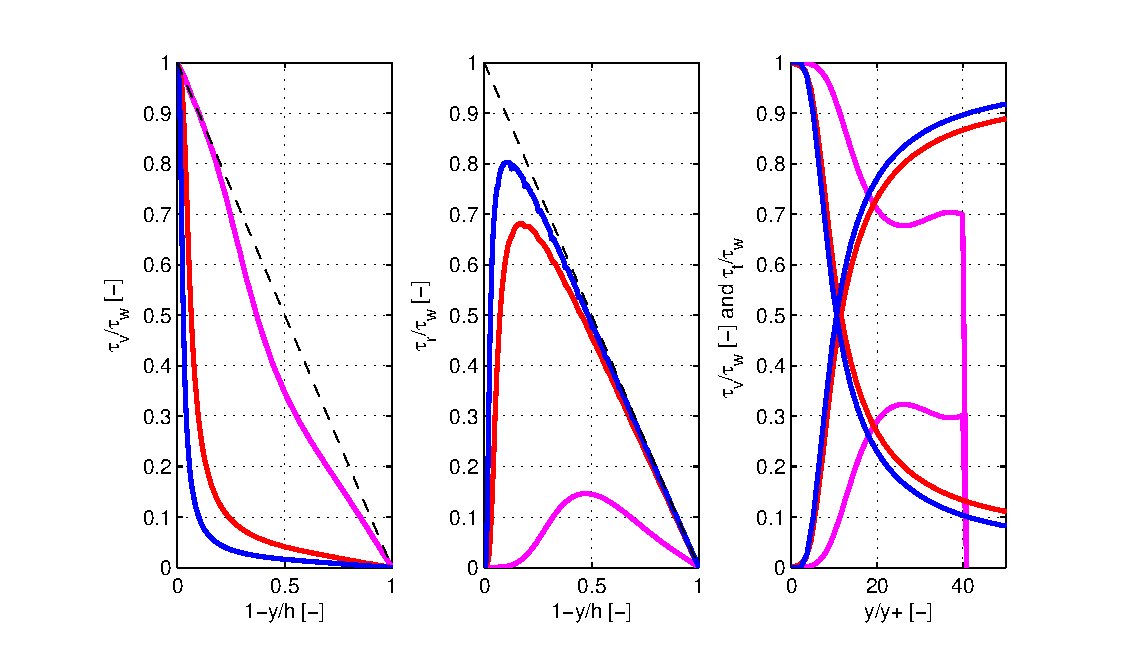
\includegraphics[width=0.8\textwidth]{FIGURES/tau.eps}
\caption{lfdjsljlfds}
\label{fig:channel-u-profile}
\end{figure} 


\noii The velocities behave as expected. In the laminar case, the velocity profile has a parabolic form with a maximum of 1.5m/s. The turbulent simulations result in lower maximum velocities (u $\le$ 1.5m/s) and a higher slope of the velocities near the wall: the results for both turbulent models are comparable (for a more detailed comparison see section~XY).

\subsubsection*{Shear stress}

Figure~\ref{fig:channel-tau} shows the shear stress profile along the cross section for each turbulent case. The shear stress components are normalized with $\tau_{net}=\tau_v+\tau_r$:

\begin{itemize}
\item viscous stress $\tau_v=\rho\nu\abl{\ave u}{y}$
\item Reynolds stress $\tau_r=-\rho\ave{u' v'}=\rho\nu_t\abl{\ave u}{y}$
\end{itemize}

\begin{figure}[!htb]
\centering
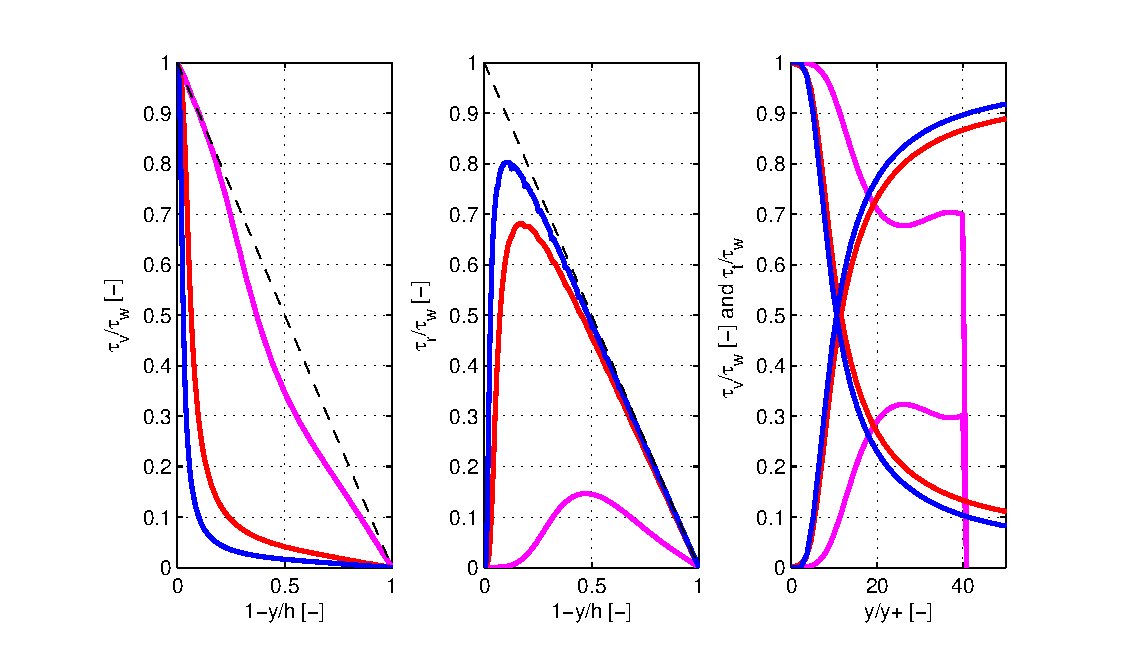
\includegraphics[width=1.0\textwidth]{FIGURES/tau.eps}
\caption{dsfdsfsdg}
\label{fig:channel-tau}
\end{figure} 

\noindent Additionally the shear stress components are plotted over $y^+$. Self-similarity is clearly recognisable.



\subsubsection{Comparison with the literature: velocity profile for Re=5600}\label{sec:lit}
Following additional values have been calculated for the turbulent Re=5600 case.
\begin{align}
u_\tau=\sqrt{\tau_w/\rho}
\qquad\qquad
l^+=\nu/u_\tau
\qquad\qquad
Re_\tau=u_\tau\cdot\delta/\nu
\end{align}
Dimensionless dimensions were created with these and were compared to the measurement values from the literature [Kim, John; Moin, Parviz; Moser, Robert: Turbulence statistics in fully developed channel flow at low Reynolds number, in: J. Fluid Mech. (1987), vol. 177, p. 133-166]:

\begin{center}
\begin{tabular}{|l|c|c|c|}
\hline
 & Literature & Algebraic & $k$-$\varepsilon$ \\\hline
$Re_\tau$ & 180 & 352 &  \\\hline
$Re_c$ & 3300 & 3329 &   \\\hline
$Re_m$ & 5600 & 5600 &  \\\hline
$u_m/u_\tau$ & 15.63 & 7.95 &  \\\hline
$u_c/u_\tau$ & 18.20 & 9.45 &  \\\hline
$u_c/u_m$ & 1.16 & 1.189 &  \\\hline
$C_f = \tau_w / (0.5 \rho u_m^2)$ & 8.18$\times$10$^{-3}$ & 31.6$\times$10$^{-3}$ &  \\\hline
\end{tabular}
\end{center}

\noindent The simulated maximal velocity $u_c/u_m$ matches well with the value from the literature for both turbulent simulations. However, all the $\tau_w$-related variables ($Re_\tau$, $C_f$, $u_\tau$...) are estimated much more precisely by the $k$-$\epsilon$-model. Apparently $\tau_w$  is overestimated by the more simpler model.

\subsubsection{Sublayers}

Figure~\ref{fig:sublayers_y+}-left shows the normalized velocity $w^+$  over $y^+$ and the expected velocity profile. They do match very well for high Reynolds-numbers: the linear sublayer is described exactly, the logarithmic layer shows slight discrepancy to the expectations.

\begin{figure}[!htb]
\centering
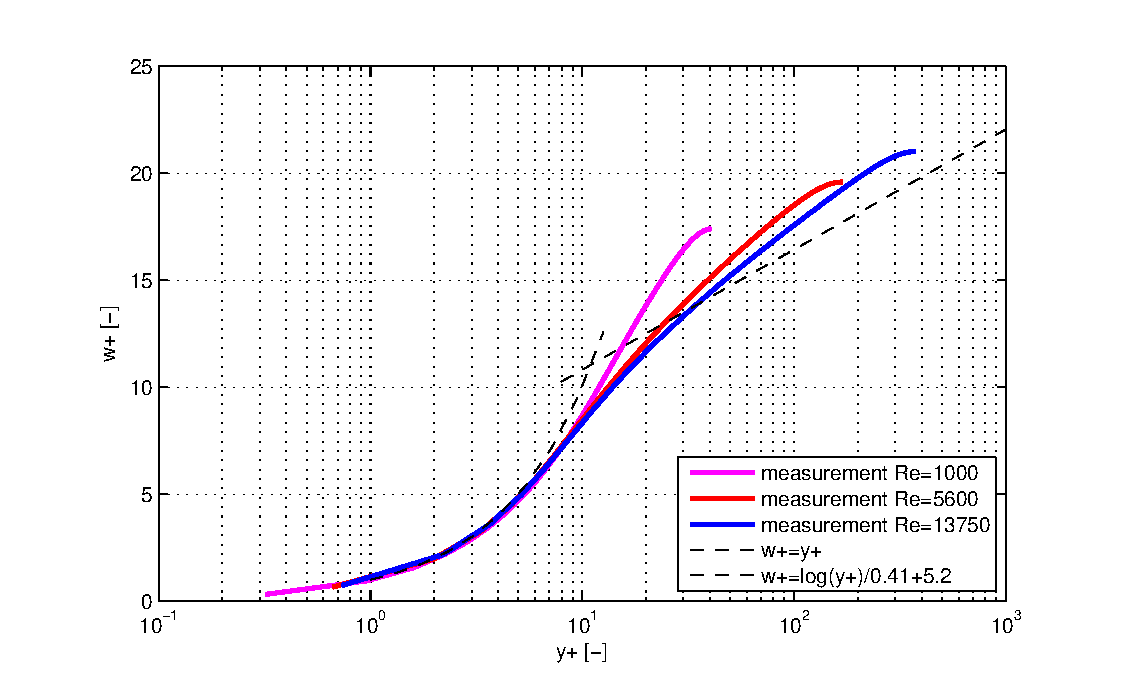
\includegraphics[width=0.9\textwidth]{FIGURES/wplusyplus.eps}
\caption{Sublayers: $w^+$ over $y^+$}
\label{fig:sublayers_y+}
\end{figure} 

\noindent Figure~\ref{fig:sublayers_y+}-right shows a modified normalized velocity $w^+$ over $y^+$ for the algebraic turbulence model for Re=5600. In this case, $l^+$ and $u_{\tau}$ was calculated with the $\tau_w$-value estimated with help of the $k$-$\varepsilon$ simulation (as discussed in section~\ref{sec:lit}). It is obvious...



%Re = 1000
%
%Re = 5600 (Kim)
%      ->$\tau_w$
%      ->$u_\tau$
%      ->$u_c$	
%
%Re = 13750 (Pope)
%	  -> TKE
	  
	  
%velocity -> re 5600 (ke und aturb)


\subsubsection*{Comparison with the literature: tke profile for Re=13750}

In the following the single terms in the $k$-transport equation are examined in more detail. The implemented form of this equation (see also XY) has the following form:

\begin{align}
\abl{k}{t} + u_i\,\abl{k}{x_i}
&=
\abl{}{x_i}\left(  B_k \abl{k}{x_i} \right) 
-
\gamma \, k
+
F
-
D
\end{align}
For a stationary fully developed channel flow the equation reduces to the following form:
\begin{align}
0
&=
\underbrace{
\abl{}{y}\left(  B_k \abl{k}{y} \right) 
}_{1}
\underbrace{
-
\gamma \, k
-
D
}_{2}
\underbrace{+
F}_3
\end{align}
with the diffusion term (1), the disspation term (2) and production term (3) being in equilibrium.
\begin{figure}[!htb]
\centering
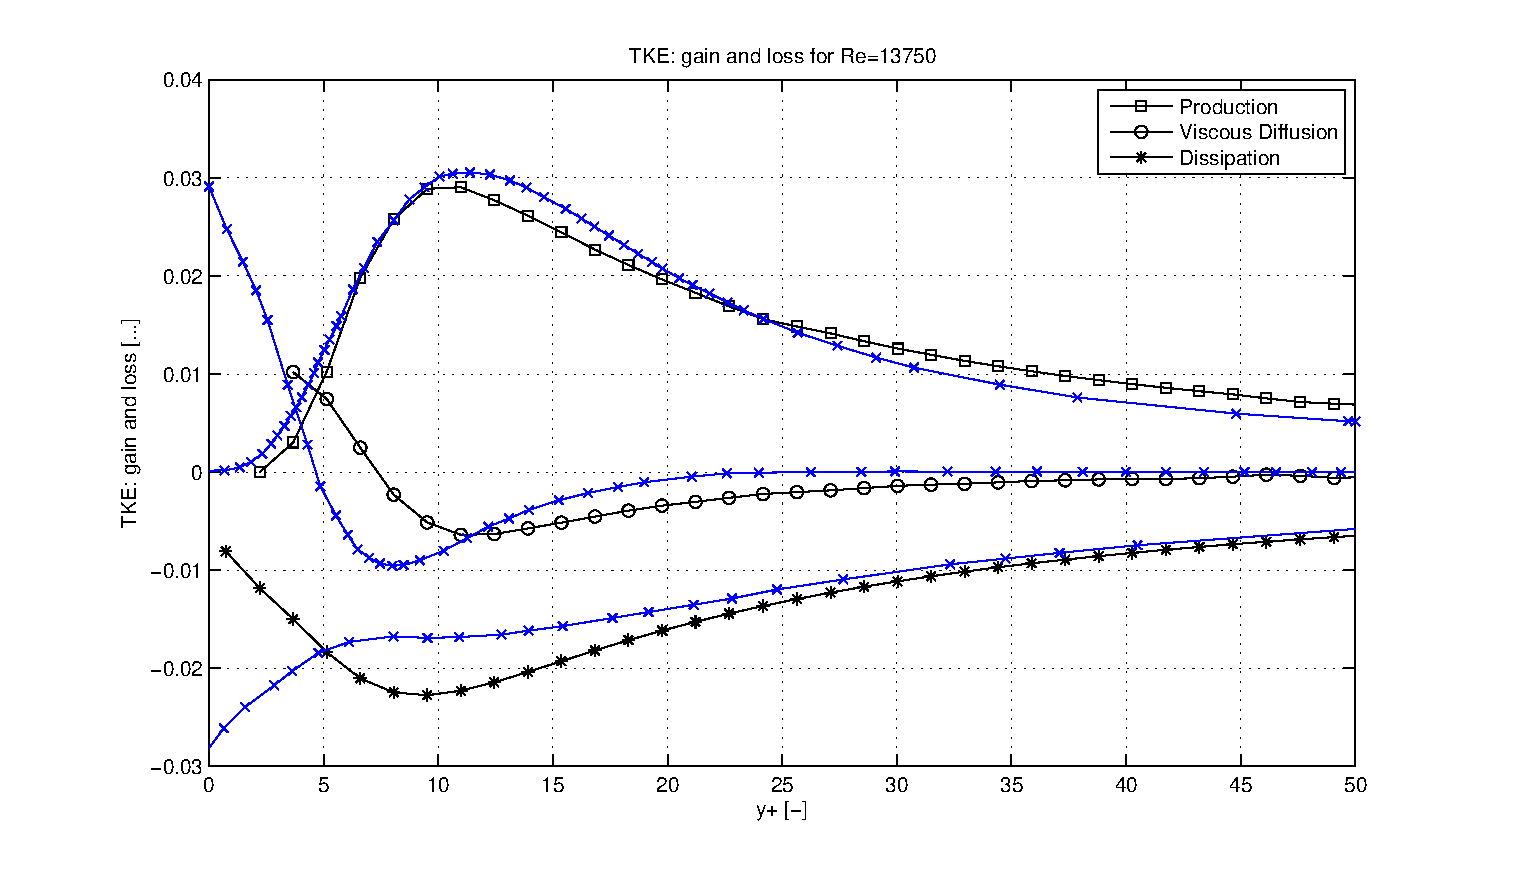
\includegraphics[trim=60 0 60 0,clip,width=0.95\textwidth]{FIGURES/tkegainloss.eps}
\caption{Terms of the TKE-transport equation for Re=13750 (in comparison with literature [Pop-90, S. 250] scaled by 0.13)}
\label{fig:circle_in_channel}
\end{figure} 

influence wall model

comparison aturb

% subsection channel_flow (end)

\newpage
\section{Boundary layer} % (fold)
\label{sec:boundary_layer}

Josef

% subsection boundary_layer (end)

% chapter validation_of_k_epsilon_model (end)